\chapter{Introdução}
O crescimento no consumo de energia cada vez mais vem aumentando conforme os anos, segundo \cite{balanco_energetico}, o
Brasil consumiu 531.1 TWh no ano de 2014, resultando em um aumento de 2.9\% comparado à 2013.

O Brasil possui uma matriz energética predominantemente renovável tendo como ênfase a geração hidráulica, as fontes renováveis correspondem à 84.1\% e não renováveis 26.9\%, conforme ilustrado na imagem \ref{consumo-2014}.

\begin{figure}[h]
    \centering
    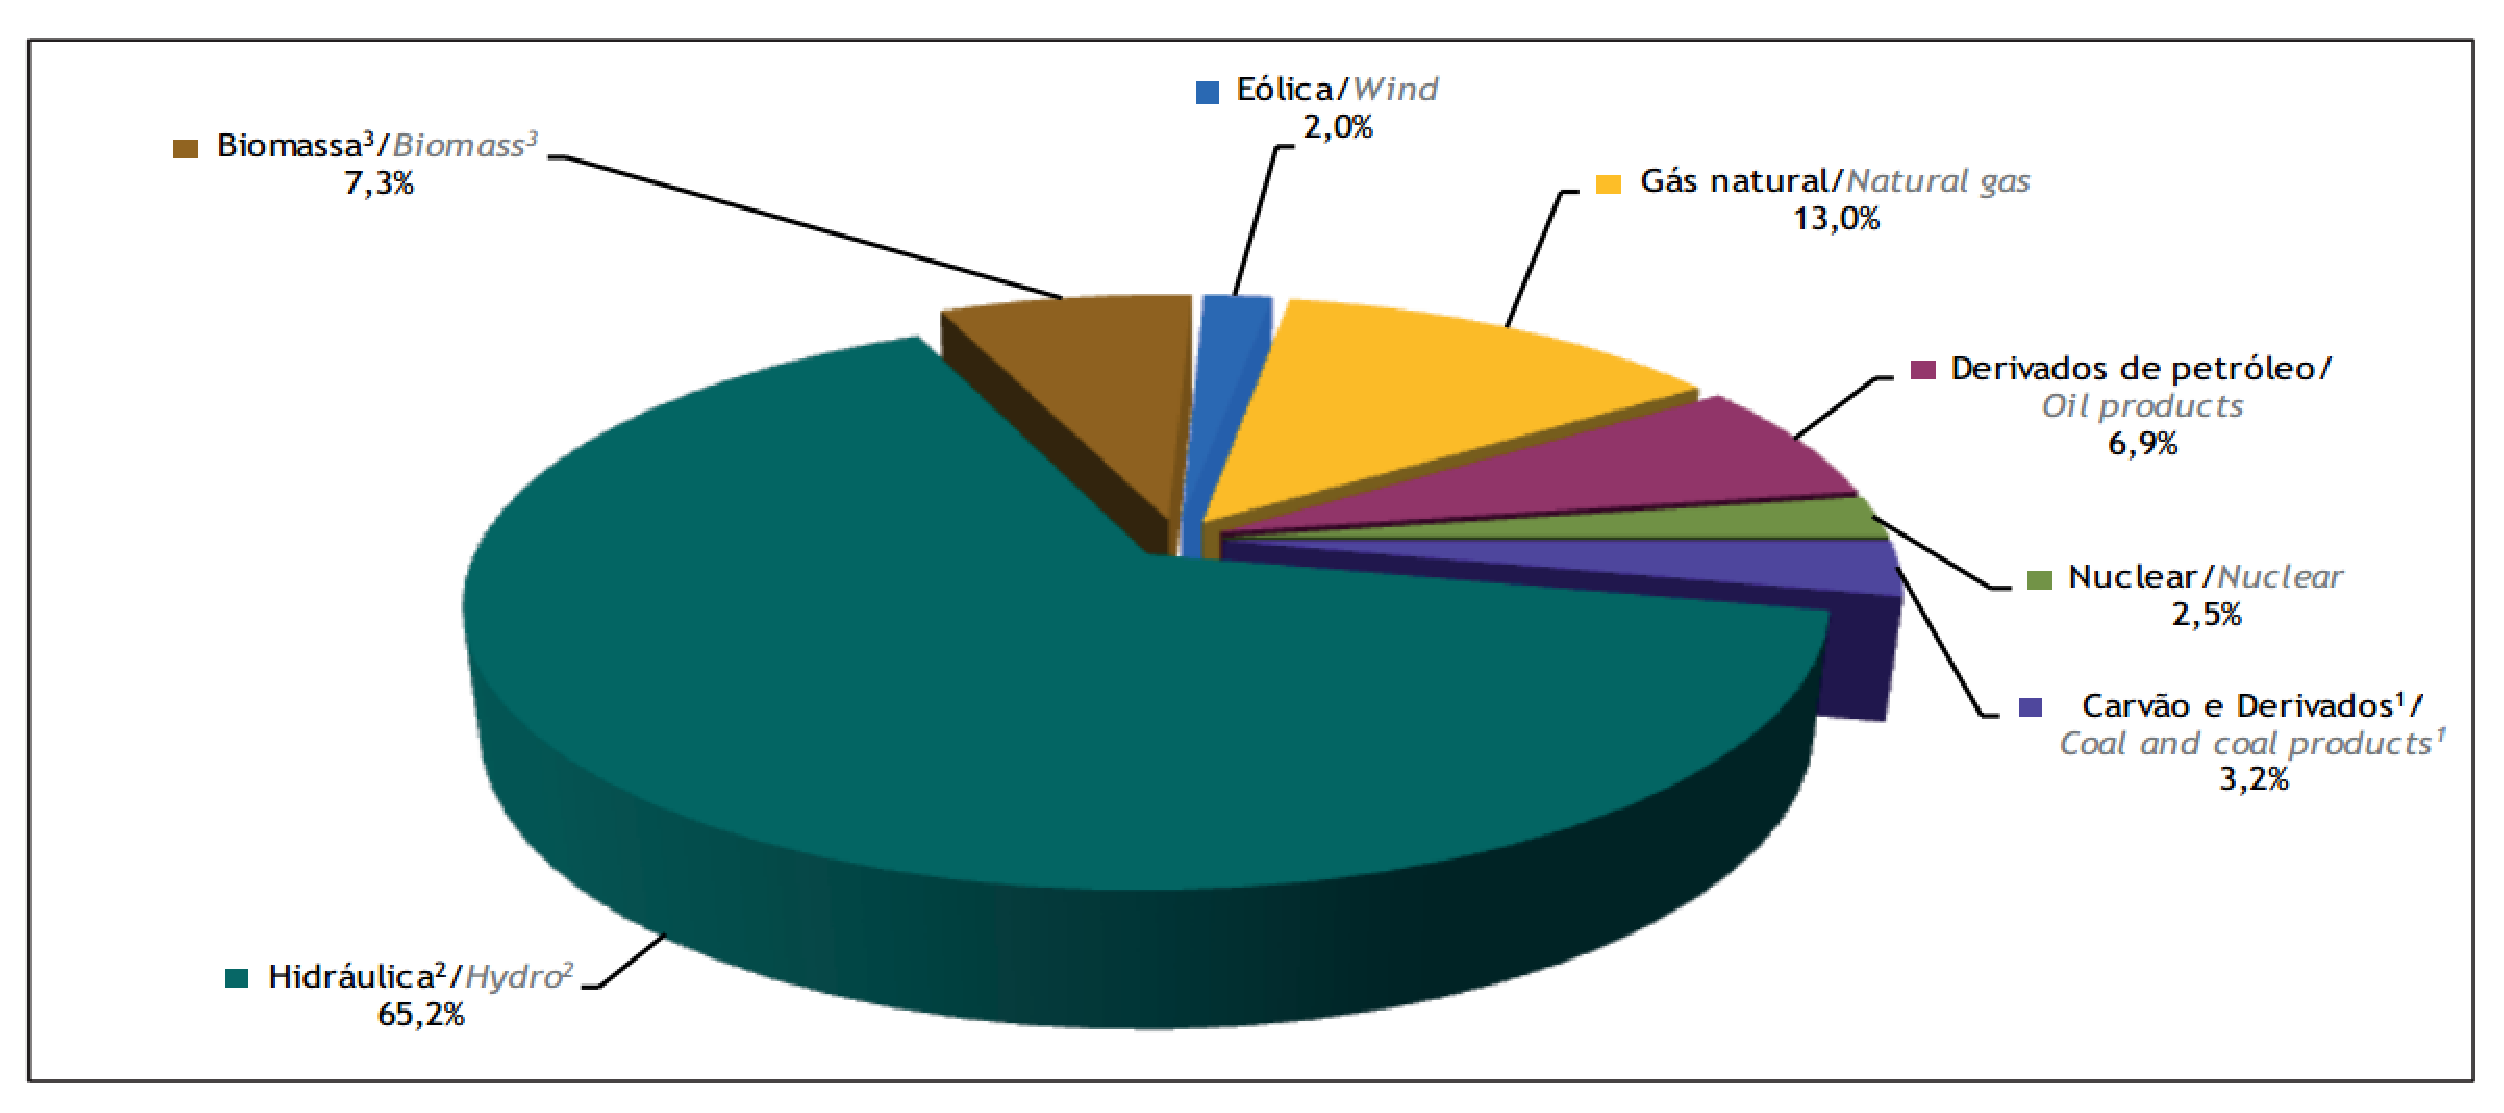
\includegraphics[keepaspectratio=true,scale=0.4]{figuras/consumo_energia_2014.eps}
    \caption{Oferta Interna de Eletricidade no Brasil em 2014}
    \label{consumo-2014}
\end{figure}

\section{Justificativa}
No ano de 2015 foi realizado um reajuste tarifário da energia elétrica correspondente à 33\% para clientes
residenciais e 32,5\% para empresas, indústrias e comércios \cite{aumento_energia}, ou seja, o uso abusivo dessa fonte
acarreta em gastos excessivos e desnecessários.

Dentre as alternativas para reduzir o consumo de energia elétrica encontram-se o uso de equipamentos mais eficientes, certificações Procel, uso racional da energia e afins, porém, quando se trata de instalações de grande porte, como Universidades e órgãos públicos em geral, percebe-se que um dos grandes problemas enfrentado é a falta de monitoramento adequado do uso de energia elétrica.

Idealiza-se que esse conhecimento de forma setorial do quanto está sendo consumido acarretará em uma analise preditiva e corretiva das instalações, visando uma maior conscientização dos usuários, consumo eficiente e economia.

A presente proposta destre trabalho encontra-se direcionada para o desenvolvimento, tendo como base os conhecimentos
adquiridos por um Engenheiro de Software, de um sistema de gerenciamento energético para uma instalação de grande porte referente à Universidade de Brasília.

\section{Objetivo Geral}
Desenvolver sistema web capaz de monitorar, em tempo real, medições de energia coletadas por transdutores
instalados em quadros de energia da Universidade de Brasília.

\subsection{Objetivos Específicos}
O sistema deve ser capaz de:
\begin{itemize}
    \item Cadastrar/Editar/Remover transdutores.
    \item Utilizar rede da universidade para comunicar-se com transdutores.
    \item Realizar a coleta de dados de forma automatizada e temporizada.
    \item Mostrar aos usuários os dados de energia coletados.
\end{itemize}

\section{Metodologia Utilizada}

\section{Estruturação do Trabalho}
